\documentclass[%
%reprint,
superscriptaddress,
%groupedaddress,
%unsortedaddress,
%runinaddress,
%frontmatterverbose,
%preprint,
showpacs,
%preprintnumbers,
nofootinbib,
%nobibnotes,
%bibnotes,
amsmath,amssymb,
aps,
%pra,
%prb,
prc,
%paper,
%rmp,
%prstab,
%prstper,
twocolumn,
floatfix ]%
{revtex4-1}

%\usepackage{acrofont}%NOTE: Comment out this line for the release version!
\newcommand{\revtex}{REV\TeX\ }
\newcommand{\classoption}[1]{\texttt{#1}}
\newcommand{\macro}[1]{\texttt{\textbackslash#1}}
\newcommand{\m}[1]{\macro{#1}}
\newcommand{\env}[1]{\texttt{#1}}
\setlength{\textheight}{9.5in}

\usepackage{comment}
\usepackage[dvips]{graphicx}
%\usepackage{amsmath,amssymb}
%\usepackage{mathrsfs}
%\usepackage{txfonts}
\usepackage{braket}
%\usepackage{latexsym}
%\usepackage{ascmac}
%\usepackage{fancybox}
%\usepackage{type1cm}
\usepackage{cases}
\usepackage{caption}
%\usepackage[top=25truemm,bottom=20truemm,left=20truemm,right=20truemm]{geometry}

  \makeatletter
    \renewcommand{\theequation}{%
    \thesection.\arabic{equation}}
    \@addtoreset{equation}{section}
  \makeatother

\begin{document}

\renewcommand{\thefootnote}{\fnsymbol{footnote}}

\title{Low-lying collective excited states in non-integrable system based on stationary phase approximation to the path integral}%

\author{Fang Ni}
 \affiliation{Faculty of Pure and Applied Sciences,
              University of Tsukuba, Tsukuba 305-8571, Japan}
\author{Takashi Nakatsukasa}
 \affiliation{Center for Computational Sciences,
              University of Tsukuba, Tsukuba 305-8577, Japan}
 \affiliation{Faculty of Pure and Applied Sciences,
              University of Tsukuba, Tsukuba 305-8571, Japan}
 \affiliation{iTHES Research Group, RIKEN, Wako 351-0198, Japan}

\begin{abstract}
\begin{description}
\item[Background] This part would describe the
context needed to understand what the paper
is about.
\item[Purpose] This part would state the purpose
of the present paper.
\item[Method] This part describe the methods
used in the paper.
\item[Results] This part would summarize the
results.
\item[Conclusions] This part would state the
conclusions of the paper.
\end{description}
\end{abstract}

\maketitle

\section{Introduction}


\section{Theoretical framework}

\subsection{One-dimensional adiabatic self-consistent collective coordinate method}
\label{ASCC}

We review the one-dimensional adiabatic self-consistent collective coordinate method (ASCC) briefly. The classical Hamilton's equation which is identical to the TDHFB equation is described by canonical variables $\{\xi^{\alpha},\pi_{\alpha}\}$. If we assume the collective motion is slow motion, it allows us to expand momenta $\pi$ up to second order. The multi-dimensional Hamiltonian is
\begin{align}
  \mathcal{H} &= V(\xi) + \frac{1}{2}B^{\alpha\beta}(\xi)\pi_{\alpha}\pi_{\beta}
\end{align}
with potential $V(\xi)$ and reciprocal mass parameter $B^{\alpha\beta}(\xi)$ defined by
\begin{align}
  V(\xi) &= \mathcal{H}(\xi,\pi=0) \\
  B^{\alpha\beta}(\xi) &= \left. \frac{\partial^2\mathcal{H}(\xi,\pi)}{\partial\pi_{\alpha}\partial\pi_{\beta}} \right|_{\pi=0}.
\end{align}
 If there is a one-dimensional collective motion which is decoupled from other intrinsic motions, the collective motion can be described by a set of canonical variable $\{q,p\}$, the one dimensional collective Hamiltonian is
\begin{align}
  \mathcal{H}_{coll} &= \bar{V}(q) + \frac{1}{2}\bar{B}^{-1}(q)p^2.
  \label{coll}
\end{align}
To obtain the collective Hamiltonian, we need to consider extended adiabatic transformation
\begin{align}
  q = q^1 &= f^1(\xi) + \frac{1}{2}f^{(1)1\alpha\beta}(\xi)\pi_{\alpha}\pi_{\beta}  \label{point}\\
 \xi^{\alpha} &= g^{\alpha}(q) + \frac{1}{2}g^{(1)\alpha 1 1}(\xi)p_{1}p_{1}
\end{align}
and
\begin{align}
  p_1 &= g_{,1}^{\alpha}\pi_{\alpha} \\
 \pi_{\alpha} &= f^1_{,\alpha}p_1 ,
  \label{momenta}
\end{align}
where the index $1$ indicates the collective degree of freedom, and the comma indicates the partial derivative $(f^1_{,\alpha}=\partial f^1/\partial \xi^{\alpha})$. 
With these relations, collective potential $\bar{V}(q)$ and collective mass parameter $\bar{B}(q)$ can be transformed by
\begin{align}
  \bar{V}(q) &= V(\xi) \\
  \bar{B}^{-1}(q) &= f^1_{,\alpha}B^{\alpha\beta}(\xi)f^1_{,\beta} ,
  \label{coll_mass}
\end{align}

Before showing the ASCC basic equations, we consider the constants of motion in TDHFB dynamics. Since nuclei is self-bound systems without external potential, the ground state obtained from mean-field theory violates the symmetry (e.g. deformation, pairing). In such system, the constants of motion corresponding the Nambu-Goldstone (NG) mode emerges in TDHFB dynamics. Therefore, we are mostly interested in the systems with collective motion separated from NG mode.\par
We know that the most of conserved quantities, such as total angular momentum $J$ and total particle number $N$, are not only expressed by one-body Hermitian operators, but also has real matrix elements in the quasi-particle basis. Such classical variable $\mathcal{P}$ corresponding to the conserved quantity can be expanded as
\begin{align}
  \mathcal{P}(\xi,\pi) = f^I(\xi) + \frac{1}{2}f^{(1)I\alpha\beta}(\xi)\pi_{\alpha}\pi_{\beta} . \label{P}
\end{align}
The index $I$ indicates the degree of freedom for NG mode. Since the conserved quantity must fulfill $\{\mathcal{P},\mathcal{H}\}_{PB}=0$, it leads
\begin{align}
  f^{I}_{,\alpha}B^{\alpha\beta} - f^{(1)I\alpha\beta}V_{,\alpha} = 0.
  \label{P_PB}
\end{align}

Including the NG mode, $f^1(\xi)$ and $g^{\alpha}(q)$ are obtained by solving ASCC basic equations 
\begin{align}
  &\delta H_M(\xi,\pi) = 0 \label{mfHFB} \\ 
  \tilde{B}^{\beta\gamma}V_{;\gamma\alpha}f^1_{,\beta}  &= \omega^2 f^1_{,\alpha},\hspace{2em} 
  \tilde{B}^{\beta\gamma}V_{;\gamma\alpha}g^{\alpha}_{,1} = \omega^2 g^{\beta}_{,1} .
  \label{mfQRPA}
\end{align}
The first equation (\ref{mfHFB}) is called moving-frame HFB equation. The moving-frame Hamiltonian $\mathcal{H}_M$ with constraints on collective coordinate and constant of motion is
\begin{align}
  \mathcal{H}_M(\xi,\pi) &= \mathcal{H}(\xi,\pi) -\lambda_1 q^1(\xi,\pi) - \lambda_I \mathcal{P}(\xi,\pi) .
\end{align}
The second equation (\ref{mfQRPA}) is called moving-frame QRPA equation. $\tilde{B}^{\alpha\beta}$ is the modified mass parameter
\begin{align}
  \tilde{B}^{\alpha\beta}(\xi) &= \frac{\partial^2 \mathcal{H}_M}{\partial\pi_{\alpha}\partial\pi_{\beta}}  \nonumber \\
&= B^{\alpha\beta}(\xi) - \lambda_I f^{(1)I\alpha\beta}(\xi) - \lambda_1 f^{(1)1\alpha\beta}(\xi) \label{tildeB}.
\end{align} 
and the covariant derivative $V_{;\gamma\alpha}$ is defined by
\begin{align}
 V_{;\alpha\beta} = V_{,\alpha\beta} - \Gamma^{\gamma}_{\alpha\beta}V_{,\gamma} , \label{covariant}
\end{align}
where the affine connection is $\Gamma^{\alpha}_{\beta\gamma}=\frac{1}{2}B^{\alpha\delta}(B_{\delta\beta,\gamma}+B_{\delta\gamma,\beta}-B_{\beta\gamma,\delta})$. If we assume that the collective coordinate $q$ is geodesic, $\tilde{B}^{\beta\gamma}V_{;\gamma\alpha}$ can be simplified after several steps
 \begin{align}
\tilde{B}^{\alpha\gamma}V_{;\gamma\beta} = \tilde{B}^{\alpha\gamma}(V_{,\gamma\beta}-\lambda_If^I_{,\gamma\beta}) + \frac{1}{2}\tilde{B}^{\alpha\gamma}_{,\beta}V_{,\gamma} 
\label{M}.
\end{align}

We discuss the practical solution to derive the one-dimensional collective coordinate. We neglect $f^{(1)1\alpha\beta}(\xi)$ because it is supposed to be negligibly small in the previous study. On the other hand, from (\ref{P_PB}) and (\ref{mfQRPA}), $f^{(1)I\alpha\beta}(\xi)$ is necessary information to promise $\tilde{B}^{\beta\gamma}V_{;\gamma\alpha}f^I_{,\beta}=0$, which means zero mode. In most of case, we know the explicit form of $\mathcal{P}(\xi,\pi)$. The procedures to obtain the collective path are (see Figure \ref{scc}): 
\begin{enumerate}
\item Find the energy minimum point in energy surface by solving (\ref{mfHFB}) (normal HFB equation). We usually set $q^1=0$ at the energy minimum point.
\item Using (\ref{M}), diagonalize (\ref{mfQRPA}) and choose the lowest mode basically\footnote{
When eigenvalues cross on the collective path, the choice of adiabatic path or diabatic path is a critical problem}. 
\item The right eigenvector $g^{\alpha}_{,1}$ tell us the direction which system moves in energy surface. Use the relation $d\xi^{\alpha}=g^{\alpha}_{,1}dq^1$ to decide the neighborhood point $q^1\to q^1+dq^1$ in the collective path. 
\item Find the non-equilibrium energy minimum point by solving (\ref{mfHFB}) at the neighborhood point, and obtain the chemical potential $\lambda_I(q)$. 
\item Iterate (2)$\sim$(4) under the same direction in energy surface. 
\item Do (2)$\sim$(5) for the opposite direction of the collective path in energy surface. 
\end{enumerate}
The scale of the collective coordinate is not unique because of the uncertainty of the eigenvectors in (\ref{mfQRPA}). To unify the scale, the simplest procedure is to keep the collective mass parameter $\bar{B}^{-1}(q)=1$ by renormalizing eigenvectors in (\ref{coll_mass}). 

\subsection{Stationary-phase approximation to the path integral}

In integrable system, we can apply the stationary phase approximation to the path integral (SPA) to obtain collective excited states. The concept of SPA is introduced in the previous study. Because the one-dimensional collective path extracted from TDHFB degrees of freedom is integrable system, SPA is supposed to be available for non-integrable system via ASCC. \par
Based on SPA, the $k$-th excited state $\ket{\psi_k}$ can be constructed by a periodic TDHFB trajectory
\begin{equation}
	\ket{\psi_k} = \oint d\mu(Z^{(k)}) \ket{Z^{(k)}}
	e^{i\mathcal{T}[Z^{(k)}]/\hbar} .
	\label{SPA}
\end{equation}
The integration indicates we integrate a periodic TDHFB trajecotry for one period in TDHFB phase space. The invariant measure $d\mu(Z)$ is defined by the unity condition $\int d\mu(Z) \ket{Z}\bra{Z} = 1$. The action integral $\mathcal{T}$ is defined by
\begin{align}
\mathcal{T}[Z] &\equiv
\int_{0}^{t} \braket{Z(t')| i\hbar\frac{\partial}{\partial t'}
	|Z(t')} dt' .
\label{tau}
\end{align}

We try to combine SPA with ASCC. The key point is to find the correspondence between TDHFB phase space and collective subspace in a TDHFB trajectory (See Fig. \ref{correspondence}). We consider the time-dependent state vector $\ket{Z(t)}$ is in a collective subspace. With pairing correlation, $\ket{Z(t)}$ can be expressed as
\begin{align}
 \ket{Z(t)} &= \ket{\Phi,J;q,p} = e^{-i\Phi \hat{J}} \ket{J;q,p} ,
 \label{GCS}
\end{align}
where $\Phi$ is the total gauge angle and $J=N/2$ is the conjugate momentum corresponding total particle number. The second equal sign indicates an intrinsic state $\ket{J;q,p}$ rotates in the gauge space. Since $[H,J]=0$, the classical Hamiltonian 
becomes
\begin{align}
 \mathcal{H} &= \braket{\Phi,J;q,p|H|\Phi,J;q,p} \nonumber \\
 &= \braket{J;q,p|H|J;q,p} \equiv \mathcal{H}_J(q,p)
\end{align}  
has no dependence of $\Phi$. Therefore, the classical Hamiltonian is the function of $(q,p)$ in a fixed particle number system, and correspond to (\ref{coll}). From ASCC, we can obtain the static state vector at each point of $q$, namely $\ket{J;q,p=0}$. To construct $\ket{J;q,p}$, we use (\ref{momenta}) at $(q,p)$ which we want to know in the collective phase space. Usually, we are interested in the points $(q^{(k)},p^{(k)})$ at the $k$-th TDHFB trajectory. Such $k$-th TDHFB trajectory is obtained from EBK quantization condition ($k$: integer)
\begin{align}
	\mathcal{T}_\circ[Z^{(k)}]=&
	\oint \braket{Z^{(k)}(t')| i\hbar\frac{\partial}{\partial t'} |Z^{(k)}(t')} dt' \nonumber \\
	=& \oint p^{(k)} dq^{(k)} = 2k\pi .
	\label{EBK}
\end{align}

\begin{figure}[htbp]
 \begin{center}
    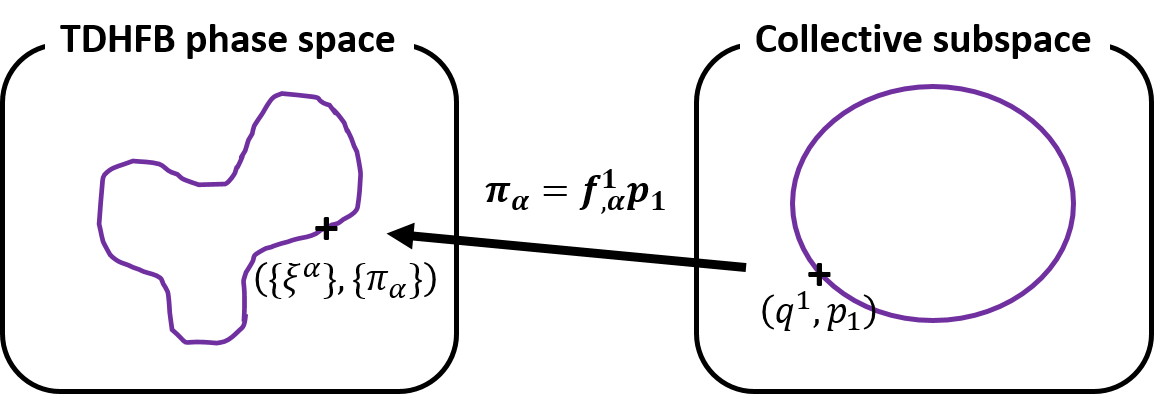
\includegraphics[width=80mm, bb=0 0 550 180]{SPA.png}
 \end{center}
  \caption{For a TDHFB trajectory, the correspondence between TDHFB phase space and collective subspace.}
  \label{correspondence}
\end{figure}

The procedures to obtain excited states from SPA via ASCC are:
\begin{enumerate}
\item Obtain the one-dimensional collective coordinate from ASCC.
\item Using collective Hamiltonian, obtain $k$-th excitation energy and TDHFB trajectory under EBK quantization condition (\ref{EBK}).
\item For $k$-th TDHFB trajectory, construct the state vector $\ket{J;q,p}$ by using (\ref{momenta}).
\item Calculate action integral (\ref{tau}) in $k$-th TDHFB trajectory.
\item Using (\ref{SPA}), obtain $k$-th excited state.
\end{enumerate}

\section{Application in pairing model}
We study the low-lying excited $0^+$ states in multi-level pairing model by applying SPA via ASCC. 
The Hamiltonian of the pairing model is given in terms of
single-particle energies $\epsilon_l$ and the pairing strength $g$ as
\begin{align}
	H &= \sum_l \epsilon_l n_l - g \sum_{l,l'} S_l^+ S_{l'}^- \nonumber \\
    &= \sum_l\epsilon_l(2S_l^0+\Omega_l) - g S^+ S^{-} ,
\end{align}
where we use the SU(2) quasi-spin operators,
$\boldsymbol{S}=\sum_l \boldsymbol{S}_l$, with
\begin{eqnarray}
        S_l^0 &=& \frac{1}{2}(\sum_ma_{lm}^{\dag}a_{lm}-\Omega_l) ,\\
        S_l^{+} &=& \sum_{m>0}a_{lm}^{\dag}a_{l\overline{m}}^{\dag} ,
\quad   S_l^{-} = S_l^{+\dag} .
\end{eqnarray}
Each single-particle energy $\epsilon_l$ possesses $(2\Omega_l)$-fold
degeneracy ($\Omega_l=j_l+1/2$)
and $\sum_{m>0}$ indicates the summation over $m=1/2,3/2,\cdots,$ and $\Omega_l-1/2$.
The occupation number of each level $l$ is given by
$
	n_l = \sum_m a^{\dag}_{lm}a_{lm} = 2S_l^0+\Omega_l ,
$.
The quasi-spin operators satisfy the commutation relations
\begin{equation}
  [S_l^0,S_{l'}^{\pm}] = \pm\delta_{ll'}S_{l}^{\pm},
	\quad [S_{l}^{+},S_{l'}^{-}] = 2\delta_{ll'}S_{l}^{0} .
\end{equation}
The magnitude of quasi-spin for each level is
$S_l=\frac{1}{2}(\Omega_l-\nu_l)$, where $\nu_l$ is the seniority
quantum number, namely the number of unpaired particle at each level $l$.
In the present study, we only consider seniority zero states with
$\nu=\sum_l \nu_l=0$.
The residual two-body interaction only consists of monopole pairing
interaction which couples two particles to zero angular momentum.
We obtain exact solutions either by solving Richardson equation
\cite{Richardson,Richardson2,Richardson3} or
by diagonalizing the Hamiltonian using the quasi-spin symmetry.

\subsection{Classical form of TDHFB Hamiltonian}
The coherent state for the seniority $\nu=0$ states
($S_l=\Omega_l/2$) is constructed as
\begin{equation}
	\ket{Z(t)} = \prod_{l} \left(1+|Z_l(t)|^2\right)^{-\Omega_l/2}
	\exp [Z_l(t) S_l^{+}] \ket{0}
 \label{coherent}
\end{equation}
where $\ket{0}$ is the vacuum (zero particle) state,
$Z_l(t)$ are time-dependent complex variables which describe
motion of the system. 
In the SU(2) quasi-spin representation,
$\ket{0}=\prod_l \ket{S_l,-S_l}$.
The coherent state $\ket{Z(t)}$ is a superposition of
states with different particle numbers
without unpaired particles.
%If $Z_l$ are all real,
In the present pairing model,
the coherent state is the same as the time-dependent BCS wave function
with $Z_l(t)=v_l(t)/u_l(t)$,
where $(u_l(t),v_l(t))$ are the time-dependent BCS $u,v$ factors.

The TDHFB equation can be derived from the time-dependent variational
principle (we set $\hbar=1$),
\begin{equation}
	\delta \mathcal{S} = 0,
	\quad
%  \delta \int \braket{\phi(t)|i\frac{\partial}{\partial t}-H|\phi(t)}dt = 0 ,
	\mathcal{S}\equiv \int \mathcal{L}(t) dt =
	\int \braket{Z(t)|i\frac{\partial}{\partial t}-H|Z(t)}dt.
  \label{TDHFB}
\end{equation}
After transformation of the complex variables $Z_l = \tan{\frac{\theta_l}{2}}e^{-i\chi_l}$  ($0\leq\theta\leq\pi$) and several steps of the derivation, the Lagrangian $\mathcal{L}$ and the expectation value of Hamiltonian become
\begin{align}
\mathcal{L}(t) = \sum_l \frac{\Omega_l}{2}
	(1&-\cos{\theta}_l)\dot{\chi_l} - \mathcal{H}(Z,Z^*) ,\\
	\mathcal{H}(Z,Z^*) \equiv \braket{Z|H|Z}& \nonumber \\
  = \sum_l \epsilon_l\Omega_l(1- \cos{\theta}_l)& - \frac{g}{4}\sum_l \Omega_l [\Omega_l(1-\cos^2{\theta}_l)+(1-\cos{\theta}_l)^2] \nonumber \\
- \frac{g}{4}\sum_{l_1\neq l_2} \Omega_{l_1}\Omega_{l_2}&\sqrt{(1-\cos^2{\theta}_{l_1})(1-\cos^2{\theta}_{l_2})}e^{-i(\chi_{l_1}-\chi_{l_2})}   .
\label{TDHFB_Hamiltonian_2}
\end{align}
Here, we choose $\chi_l$ as canonical coordinates. Their conjugate momenta
are given by
\begin{align}
  j_l\equiv \frac{\partial\mathcal{L}}{\partial\dot{\chi}_l}=\frac{\Omega_l}{2}
	(1-\cos{\theta}_l) .
\end{align}
$\chi_l$ represent a kind of gauge angle of each level,
and $j_l$ are related to the occupation number of each level, $2j_l=n_l$. Therefore, the TDHFB Hamiltonian can be represented by canonical variables $\mathcal{H}(Z,Z^*) = \mathcal{H}(\{\chi_l\},\{j_l\})$, and the TDHFB equation is equivalent to the Hamilton's equation
\begin{equation}
	\dot{\chi_l} = \frac{\partial\mathcal{H}}{\partial j_l}, \quad
	\dot{j_l} = -\frac{\partial\mathcal{H}}{\partial \chi_l} .
\end{equation}
.

\subsection{Application into ASCC}
We construct 1D collective subspace from ASCC theory. Because the first order with respect to $\chi_l$ is zero in TDHFB Hamiltonian, we assume $j_l$ as coordinates and $\chi_l$ as conjugate momenta. The canonical variables are $(j_l,-\chi_l)$ and fulfill $\{j_l,-\chi_l'\}_{PB}=\delta_{ll'}$. We expand the classical Hamiltonian up to second order with respect to $\chi_l$. 
The classical Hamiltonian becomes
\begin{align}
  \mathcal{H}(\{\chi_l\},\{\pi_l\}) \approx& V(j) + \frac{1}{2}B^{\alpha\beta}(j)\chi_{\alpha}\chi_{\beta},
\end{align}
where potential $V(j)$ and reciprocal mass parameter $B^{\alpha\beta}(j)$ are defined as
\begin{align}
  V(j) =& \mathcal{H}(\chi=0,j) \nonumber \\
	=& \sum_l 2\epsilon_lj_l - g\sum_l \left( \Omega_lj_l - j_l^2 +\frac{j_l^2}{\Omega_l} \right) \nonumber \\
  &- g\sum_{l_1\ne l_2} \sqrt{j_{l_1}j_{l_2}(\Omega_{l_1}-j_{l_1})(\Omega_{l_2}-j_{l_2})} 	
\end{align}
\begin{align}
  B^{\alpha\beta}(j) =& \left. \frac{\partial^2\mathcal{H}}{\partial\chi_{\alpha}\partial\chi_{\beta}} \right|_{\chi=0} \nonumber \\
	=& \left\{
	\begin{array}{c}
	2g\sum_{l\ne \alpha} \sqrt{j_{l}j_{\alpha}(\Omega_{l}-j_{l})(\Omega_{\alpha}-j_{\alpha})} \hspace{2em} (\alpha=\beta) \\
	-2g\sqrt{j_{\alpha}j_{\beta}(\Omega_{\alpha}-j_{\alpha})(\Omega_{\beta}-j_{\beta})} \hspace{2em} (\alpha\ne\beta)
	\end{array}
	\right. .
 \label{mass}
\end{align}
Using the TDHFB Hamiltonian, we can apply ASCC explained in Sec. \ref{ASCC} by replacing $\xi\to j$ and $\pi\to-\chi$.

We consider the treatment for the constant of motion in pairing model. In the TDHFB Hamiltonian, there is no dependence about the total gauge angle
\begin{align}
  \Phi = \frac{1}{L}\sum_l \chi_l.
  \label{total_gauge}
\end{align}
It indicates the conjugate momentum 
\begin{align}
  J \equiv \frac{\partial\mathcal{L}}{\partial\dot{\Phi}}=\sum_l j_l = \frac{N}{2}
  \label{J}
\end{align}
is conserved quantity. From this equation, we can find $J$ is not dependent of $\chi$, which means $f^{(1)I\alpha\beta}$ in (\ref{P}) is zero. Therefore, $B^{\beta\gamma}V_{;\gamma\alpha}f^I_{,\beta}=0$ is promised exactly. Also, the second derivative of $J$ with respect to $j$ vanishes, which indicates $f^{I}_{,\gamma\beta}$ in (\ref{M}) is zero. It indicates the chemical potential $\lambda_I(q)$ is not necessary information to calculate the matrix element in moving-frame QRPA equation.

With the properties of the constant of motion, we discuss the practical solution of ASCC in pairing model. If we ignore the higher order term $f^{(1)1\alpha\beta}$, we can practice local harmonic equation (LHE)
\begin{align}
  B^{\beta\gamma}V_{;\gamma\alpha}f^1_{,\beta}  &= \omega^2 f^1_{,\alpha},\hspace{2em} 
  B^{\beta\gamma}V_{;\gamma\alpha}g^{\alpha}_{,1} = \omega^2 g^{\beta}_{,1},
  \label{LHE}
\end{align}
which simplifies the moving-frame QRPA equation (\ref{mfQRPA}) by replacing $\tilde{B}^{\beta\gamma}$ into $B^{\beta\gamma}$. Under (\ref{LHE}), the eigenvalue of spurious mode corresponding pairing rotation is exact zero. To guarantee the state vectors $\ket{Z(q)}$ are in the same total gauge angle $\Phi(q)=-\frac{1}{L} p_1\sum_l f^1_{,l}=0$, we correct the eigenvectors by
\begin{align}
  f^1_{,\alpha} \to f^1_{,\alpha} - \frac{1}{L}\sum_l f^1_{,l} 
  \label{f}
\end{align}
after solving (\ref{LHE}) at each point of $q$.

\subsection{Application into SPA}
We derive the explicit form of excited states in (\ref{SPA}). From (\ref{GCS}) and (\ref{J}), the state vector $\ket{\Phi,J;q,p}$ becomes
\begin{align}
  \ket{\Phi,J;q,p} &= \sum_{\{j_l\}} e^{-i\Phi \sum_l j_l} \ket{J;q,p} .
\end{align}
Here, $\ket{J;q,p}$ can be expanded in SU(2) quasispin basis
\begin{align}
  \ket{J;q,p} &= \sum_{\{j_l\}} A_{j_l}(q,p) \ket{\cdots;S_l,-S_l+k_l,\cdots}, 
\end{align}
where 
\begin{align}
  A_{j_l}(q,p) =& \prod_l \left(\frac{1-\cos{\theta}_l}{2}\right)^{j_l/2}\left(\frac{1+\cos{\theta}_l}{2}\right)^{(\Omega_l-j_l)/2}
  \nonumber \\
  &\times\sqrt{\frac{(\Omega_l)!}{j_l!(\Omega_l-j_l)!}} e^{-ij_l\chi_l} 
\end{align}
is in fixed gauge angle ($\Phi=0$).

Due to $J$ is conserved quantity, the action integral can be divided into two terms
\begin{align}
  \mathcal{T}(\Phi,J;q,p) &= \mathcal{T}_{\rm intr}(t) + J\Phi, 
\end{align}
where the intrinsic action integral $\mathcal{T}_{\rm intr}(t)$ becomes
\begin{align}
  \mathcal{T}_{\rm intr}(t) &= \int \braket{J;q,p|i\frac{\partial}{\partial t}|J;q,p} dt
	 \nonumber \\
	&= \int \sum_l j_l d\chi_l .
	\label{tau}
\end{align}
The important point is $\mathcal{T}_{\rm intr}(t) \ne \int p dq$ at each $t$. For closed TDHFB trajectory, only $\mathcal{T}_{\rm intr}(t)$ contributes to the excited states.
In SU(2) representation, the invariant measure is
\begin{align}
  d\mu(Z) &= \prod_l \frac{\Omega_l+1}{\pi} (1+|Z_l|^2)^{-2} d{\rm Re}Z d{\rm Im}Z \nonumber \\
 =& \prod_l \frac{\Omega_l+1}{4\pi} d \cos{\theta_l} d\chi_l \nonumber \\
 =& \prod_l \frac{-(1+\Omega_l^{-1})}{2\pi} d\chi_l dj_l \nonumber \\
 =& \left[ \prod_l \frac{-(1+\Omega_l^{-1})}{2\pi} \right] d\Phi dJ dqdp \nonumber \\
 &\times dQ_1\cdots dQ_{l-2}dP_1\cdots dP_{l-2}
% d\Phi dJ dq dp = d\Phi dJ dE dt 
\end{align}
where $(Q_i,P_i)$ are the other canonical variables decoupled from the collective coordinates. From the third line to the forth line, we used that Jacobian equals one in canonical transformation. The part of the invariant measure which contributes to the excited states is
\begin{align}
d\mu(\Phi,J;q,p) \propto d\Phi dJ dqdp = d\Phi dJ dE dt. 
\end{align}
Under EBK quantization condition (\ref{EBK}),
the $k$-th excited state becomes
\begin{align}
 \ket{\tilde{\phi}_k} \propto& \oint d\Phi \oint dt \ket{\Phi,J;q,p} e^{i\mathcal{T}(\Phi,J;q,p)}
 \nonumber \\
 =& \sum_{\{j_l\}} \oint d\Phi e^{i(J-\sum_l j_l)\Phi} \nonumber \\
 &\times \oint dt e^{i\mathcal{T}_{\rm intr}(t)} A_{j_l}(q,p) \ket{\cdots;S_l,-S_l+j_l,\cdots} \nonumber \\
 \equiv& \sum_{\{j_l\}\in (\sum_{j_l}=J)} C_{j_l} \ket{\cdots;S_l,-S_l+j_l,\cdots}
 \label{SPA2}
\end{align}
where
\begin{align}
  C_{j_l} = \oint dt e^{i\mathcal{T}_{\rm intr}(t)} A_{j_l}(q(t),p(t)).
  \label{coef}
\end{align}

The definition of wave function in SPA can also be extended into ground state. The ground state is constructed by only energy minimum point in TDHFB phase space. In the energy minimum point, $\ket{\Phi,J;q,p}=\ket{\rm HFB}$. Therefore, (\ref{SPA2}) becomes
\begin{align}
 \ket{\tilde{\phi}_{g.s.}} \propto& \sum_{\{j_l\}} \oint d\Phi e^{i(J-\sum_l j_l)\Phi} \ket{\rm HFB},  
\end{align}
which is identical to the wave function of the particle number projection for HFB state.

\section{Results}
We apply ASCC + SPA to study the multi-level system in pairing model. The TDHFB degrees of freedom equals the number of single particle levels, including the constant of motion (pairing rotation). First, we confirm the dynamics is identical between ASCC + SPA and adiabatic TDHFB in two-level (one-dimensional TDHFB) system. Next, we discuss the dynamics in non-integrable (more than three-level) system.  


\subsection{Confirmation in one-dimensional TDHFB system}
In two-level system, the classical Hamiltonian in (\ref{TDHFB_Hamiltonian_2}) is
\begin{align}
\mathcal{H} 
  =& \sum_{l=1,2} \epsilon_l\Omega_l(1- \cos{\theta}_l)& \nonumber \\ 
 &- \frac{g}{4}\sum_{l=1,2} \Omega_l [\Omega_l(1-\cos^2{\theta}_l)+(1-\cos{\theta}_l)^2] \nonumber \\
- \frac{g}{2} \Omega_{1}\Omega_{2}&\sqrt{(1-\cos^2{\theta}_{l_1})(1-\cos^2{\theta}_{l_2})}\cos{(\chi_{2}-\chi_{1})}   .
\end{align}
If we define the canonical coordinate $\phi=\chi_2-\chi_1$, it attributes to one-dimensional system. The conjugate momentum is $j= \frac{\partial\mathcal{L}}{\partial\dot{\phi}} = \{\Omega_2(1-\cos{\theta}_2) - \Omega_1(1-\cos{\theta}_1)\}/4$. The adiabatic TDHFB (ATDHFB) means that we expand the Hamiltonian with respect to $\chi$ up to second order
\begin{align}
  \mathcal{H}(\phi,j) &\approx V(j) + \frac{1}{2}B^{-1}(j)\phi^2,
\end{align}
where $V(j)=\mathcal{H}(\phi=0,j)$ and $B^{-1}(j)= \left. \frac{\partial^2\mathcal{H}}{\partial\phi^2} \right|_{\phi=0}$.
Because the time-dependent pairing vibrational mode is explicitly decoupled from pairing rotational mode, ASCC must be identical with ATDHFB. Furthermore, the excited states from SPA are also identical from both approaches.

We study the system with equal degeneracy $\Omega_1=\Omega_2=50$, $g/(\epsilon_2-\epsilon_1)=0.02$, and $N=100$. In ASCC calculation, we set the mesh size of collective coordinate $dq=0.02$. We compared the excited $0^+$ states from one-dimensional ATDHFB and ASCC with each other. Fig. \ref{fig:N100_traj} and Fig. \ref{fig:N100_tau} show the TDHFB trajectory in phase space and  action integral $\mathcal{T}$ as a function of time $t$, corresponding to $\ket{0_2^+}$, respectively. All of the mesh points obtained from ASCC are on the trajectory obtained from ATDHFB. The obtained excited $0^+$ states from SPA are shown in Fig. \ref{fig:N100_occ}. The occupation probability can be decomposed into $2n$-particle-$2n$-hole components. We can find the results from ATDHFB and ASCC are identical for all states. Therefore, the theoretical framework of ASCC + SPA has no problem.



\begin{figure}[thb]
 \begin{center}
   \includegraphics[height=0.45\textwidth,angle=-90]{N100Xeq2trajectory.eps}
 \end{center}
\caption{TDHFB trajectory of $\ket{0_2^+}$ in two-dimensional phase space. Solid line is obtained from one-dimensional ATDHFB+SPA calculation and cross points corresponding to each mesh point are obtained from ASCC+SPA. }
\label{fig:N100_traj}
\end{figure}
\begin{figure}[thb]
 \begin{center}
   \includegraphics[height=0.5\textwidth,angle=-90]{N100Xeq2tau.eps}
 \end{center}
\caption{Action integral of  $\ket{0_2^+}$ with respect to time $t$. Solid line is obtained from one-dimensional ATDHFB+SPA calculation and cross points corresponding to each mesh point are obtained from ASCC+SPA. Dashed line is $2\pi$ corresponding to $\ket{0_2^+}$ in EBK quantization condition. Based on Fig. \ref{fig:N100_traj}, we calculated the action integral from $(\phi,j)=(0,-8)$ in clockwise direction. }
\label{fig:N100_tau}
\end{figure}
\begin{figure}[thb]
 \begin{center}
   \includegraphics[height=0.5\textwidth,angle=-90]{N100Xeq2occ.eps}
 \end{center}
	\caption{Occupation probability in excited $0^+$ states
as a function of $j$ for $\Omega_1=\Omega_2=50$, $N=100$, and $x=2$ system.
The two vertical bars at each $j$ from the left to the right represent
the squared components of the wave functions
from ATDHFB+SPA and ASCC+SPA calculations, respectively.
The left end of the horizontal axis at $j=j_{\rm min}$
corresponds to a component with $(n_1,n_2)=(N,0)$.
The next at $j=j_{\rm min}+1$ corresponds to the one with
$(n_1,n_2)=(N-2,2)$, and so on.
}
 \label{fig:N100_occ}
\end{figure}


\subsection{Three-level system}
The simplest non-integrable system is three-level system. We have one trivial motion and two time-dependent degrees of freedom. We study the system with $\Omega_1=\Omega_2=\Omega_3=8$, $\epsilon_1=-1$, $\epsilon_2=0$, $\epsilon_3=1.5$, and $g=0.2$. The phase transition occurs at $g_c=0.058$ when $N=2\Omega_1=16$. We consider the even particle number chain from $N=14$ to $N=24$. 

From moving-frame QRPA equation, we obtain three modes along the collective path (Fig. \ref{omega_sq}). Except zero mode, we choose the lowest mode as collective motion. Fig. \ref{occ_number} and Fig. \ref{potential} are occupation number in each single-particle level and collective potential in the collective path, respectively. We can find the occupation numbers become to integer at both end points. Furthermore, Hartree-Fock states always emerge at one of the end point. 


\begin{figure*}[t]
 \begin{center}
  \includegraphics[width=40mm,angle=-90]{omega_sq.eps}
 \end{center}
	\caption{Eigenvalues of moving-frame QRPA equation with respect to the collective coordinate $q$, from $N=14$ to $N=24$. Purple lines are spurious modes and green lines are chosen modes corresponding to the collective coordinate. In each panel, both edges correspond to the end points of the collective coordinate.
}
 \label{omega_sq}
\end{figure*}
\begin{figure*}[t]
 \begin{center}
  \includegraphics[width=40mm,angle=-90]{occ_number.eps}
 \end{center}
	\caption{Occupation numbers in each single-particle level with respect to the collective coordinate $q$, from $N=14$ to $N=24$. At the left end point of the collective coordinate in each panel, the configurations correspond to Hartree-Fock states.
}
 \label{occ_number}
\end{figure*}
\begin{figure}[htbp]
 \begin{center}
  \includegraphics[width=60mm,angle=-90]{potential.eps}
 \end{center}
	\caption{Collective potential obtained from ASCC. We adjusted the energy minimum point as $V=0$.
}
 \label{potential}
\end{figure}

Based on the information from ASCC calculation, we can obtain the excited states from SPA.
Table \ref{ex} shows the excitation energies of first and second excited states in the collective subspace. Up to the second excitation, all of the energies are in their energy pockets shown in Fig. \ref{potential}. Comparing the result from ASCC+SPA with exact solution, we can find all of the values are nicely reproduced. The slightly difference is that the values from ASCC+SPA are about $5\%$ smaller than exact solution. 
Using the wave function of excited states, the pair additional transition strength is shown in Fig. \ref{3levelPad}. For intraband transition, comparing ASCC+SPA with exact solution, $B(P_{\rm ad};0\rightarrow 0)$ are almost identical and $B(P_{\rm ad};1\rightarrow 1)$ are about $10\%\sim20\%$ small. 
For interband transition, the strength from ASCC+SPA is much smaller than exact solution. However, because the pairing correlation is enough strong in this case, the strength of intraband transition is dominant compared with interband transition. We can find that $B(P_{\rm ad};0\rightarrow 1)$ and $B(P_{\rm ad};1\rightarrow 0)$ are only about $1\%$ of $B(P_{\rm ad};0\rightarrow 0)$ and $B(P_{\rm ad};1\rightarrow 1)$. Therefore, the interband transition can be regarded as reasonable. From all above results, we can conclude that ASCC+SPA reproduces exact solution quantitatively. 
\begin{table}[htbp]
\begin{ruledtabular}
\begin{tabular}{c|c|cccccc}
            & $N$ & $14$ & $16$ & $18$ & $20$ & $22$ & $24$\\ \hline
$0_2^+$ one & Exact & $4.09$ & $4.13$ & $4.20$ & $4.30$ & $4.44$ & $4.60$\\
phonon &ASCC+SPA & $3.87$ & $3.90$ & $3.97$ & $4.09$ & $4.23$ & $4.33$\\ \hline
$0_4^+$ two & Exact & $7.65$ & $7.71$ & $7.88$ & $8.15$ & $8.49$ & $8.74$\\
phonon &ASCC+SPA & $7.42$ & $7.42$ & $7.60$ & $7.92$ & $8.26$ & $8.47$\\
\end{tabular}
\end{ruledtabular}
\caption{Excitation energies of one-phonon and two-phonon states from exact solution and ASCC+SPA calculation. In a chosen collective subspace, one-phonon and two-phonon states correspond to the first and second excitation, respectively. In the whole Hilbert space, one-phonon and two-phonon states correspond to $\ket{0_2^+}$ and $\ket{0_4^+}$, respectively.}
\label{ex}
\end{table}

\begin{figure}[htbp]
 \begin{center}
  \includegraphics[width=60mm,angle=-90]{intra_trans.eps}
 \end{center}
 \begin{center}
  \includegraphics[width=60mm,angle=-90]{inter_trans.eps}
 \end{center}
	\caption{The strength of pair additional transition
$B(P_{\rm ad};k\rightarrow k')=|\braket{N+2,k'|S^+|N,k}|^2$, from $N=14$ to $N=22$. Dashed lines are exact solution and solid lines are ASCC+SPA calculation. Horizontal line shows the particle number of the initial states. Upper panel shows the intraband transitions of
$\ket{0_1^+}\to\ket{0_1^+}$ and $\ket{0_2^+}\to\ket{0_2^+}$,
while lower panel shows the interband transition of
$\ket{0_1^+}\to\ket{0_2^+}$ and $\ket{0_2^+}\to\ket{0_1^+}$.
}
 \label{3levelPad}
\end{figure}

\subsection{Pb isotopes}
With pairing model, we study neutron's pairing vibration in Pb isotope. We prepare the neutron's single-particle level between the magic number 82 and 126 (Table \ref{Pb}). The coupling constant $g=0.138$ is determined to reproduce the experimental pairing gap $\Delta(N)=\frac{(-1)^{N+1}}{2}(B(N+1)-2B(N)+B(N-1))$ of ${}^{192}$Pb. We consider the even-even system from ${}^{188}$Pb to ${}^{194}$Pb.
\begin{table}[htbp]
\begin{ruledtabular}
\begin{tabular}{c|cccccc}
  orbit& $h_{9/2}$ & $f_{7/2}$ & $i_{13/2}$ & $p_{3/2}$ & $f_{5/2}$ & $p_{1/2}$\\ \hline
  energy& $-10.94$ & $-10.69$ & $-8.74$ & $-8.44$ & $-8.16$ & $-7.45$\\
\end{tabular}
\end{ruledtabular}
\caption{Single-particle levels of Pb isotopes used in the calculation. The orbits are obtained from spherical Woods-Saxon potential with spin-orbit coupling. }
\label{Pb}
\end{table}

We have six TDHFB degrees of freedom in the system. Fig. \ref{Pb_omega_sq} shows the eigenvalue of moving-frame QRPA equation. We can find there are one spurious mode and five vibrational modes. Even though the degrees of freedom increase compared with three-level system, the collective modes we focus on did not cross with other modes in all panels. It means that the collective mode is nicely decoupled from other degrees of freedom. Under the chosen mode, the occupation number is shown in Fig. \ref{Pb_occ_number}. As with three-level system, the left end points correspond to HF state in all panels. The last neutrons are in $i_{13/2}$ from ${}^{188}$Pb to ${}^{194}$Pb. In the collective path, we can find $i_{13/2}$ and $p_{3/2}$ changes significantly, while other orbits are almost constant.


\begin{figure*}[t]
 \begin{center}
  \includegraphics[width=40mm,angle=-90]{Pbomega_sq.eps}
 \end{center}
	\caption{The same as Fig. \ref{omega_sq} but for Pb isotopes.
}
 \label{Pb_omega_sq}
\end{figure*}


\begin{figure*}[t]
 \begin{center}
  \includegraphics[width=40mm,angle=-90]{Pbocc_number.eps}
 \end{center}
	\caption{The same as Fig. \ref{occ_number} but for Pb isotopes.
}
 \label{Pb_occ_number}
\end{figure*}

\begin{table}[htbp]
\begin{ruledtabular}
\begin{tabular}{c|cccccc}
   & ${}^{186}$Pb & ${}^{188}$Pb & ${}^{190}$Pb & ${}^{192}$Pb & ${}^{194}$Pb & ${}^{196}$Pb\\ \hline
 Exact & $2.58$ & $2.44$ & $2.34$ & $2.25$ & $2.20$ & $2.15$\\
ASCC+SPA & unbound & $2.31$ & $2.21$ & $2.12$ & $2.04$ & unbound \\ 
\end{tabular}
\end{ruledtabular}
\caption{The same as Table. \ref{ex} but for Pb isotopes.}
\label{Pb_ex}
\end{table}

\begin{figure}[htbp]
 \begin{center}
  \includegraphics[width=60mm,angle=-90]{Pbintra_trans.eps}
 \end{center}
 \begin{center}
  \includegraphics[width=60mm,angle=-90]{Pbinter_trans.eps}
 \end{center}
	\caption{The same as Fig. \ref{3levelPad} but for Pb isotopes.
}
 \label{PbPad}
\end{figure}


\section{Conclusion}


\end{document}

